%!TEX program = xelatex
%% Copyright (C) 2024 傅祉珏
%% 
%% This file contains LaTeX source code for the Homework4 of YatML,
%% released under AGPLv3 license.
%% Full license text available in LICENSE file at project root,
%% with additional restrictions in ADDITIONAL_TERMS.md.
%% 
%% Commercial use prohibited. Academic use requires retention of this notice.
%% Source repository: https://github.com/Billiefu/YatML

% SPDX-FileCopyrightText: 2024 傅祉珏
% SPDX-License-Identifier: AGPL-3.0-or-later
% SPDX-Additional-Clauses: see ADDITIONAL_TERMS.md

\documentclass[a4paper, utf8]{ctexart}
\usepackage[fontset=Fandol]{ctex}
\usepackage{draftwatermark}
\usepackage{anyfontsize}
\usepackage{indentfirst}
\usepackage{subcaption}
\usepackage{enumitem}
\usepackage{tabularx}
\usepackage{fancyhdr}
\usepackage{geometry}
\usepackage{graphicx}
\usepackage{abstract}
\usepackage{amsmath}
\usepackage{lipsum}

\geometry{a4paper,left=31mm,right=31mm,top=25mm,bottom=25mm}
\CTEXsetup[format={\Large \bfseries}]{section}
\setlength{\parindent}{2em}
\renewcommand{\figurename}{Fig}
\renewcommand{\refname}{References}
\renewcommand{\tablename}{Table}
\pagestyle{fancy}
\fancyhf{}
\fancyhead[C]{}
\fancyhead[L]{HOMEWORK4:\ Support\ Vector\ Machine}
\fancyhead[R]{21307210\ 傅祉珏}
\fancyfoot[C]{\thepage}
\fancyfoot[L,R]{}

\setCJKfamilyfont{zhsong}[AutoFakeBold = {2.17}]{SimSun}
\renewcommand*{\songti}{\CJKfamily{zhsong}}

\title{\songti \Large \textbf{HOMEWORK4:\ Support\ Vector\ Machine}}
\author{Student\ ID:\ 21307210 \qquad Student\ Name:\ 傅祉珏}
\date{Lectured\ by\ 梁上松,\ Sun\ Yat-sen\ University}

\SetWatermarkText{Copyright\ \copyright\ 2024\ 傅祉珏}
\SetWatermarkScale{0.4}
\SetWatermarkAngle{45}
\SetWatermarkColor[gray]{0.8}

\begin{document}
	
	\maketitle
	
	\renewcommand{\abstractname}{\large \textbf{Abstract}}
	\begin{abstract}
		SVM, a non-parametric classification model, focuses on finding the best hyperplane to maximize class separation. It employs kernel functions to handle non-linear data by transforming it into a higher-dimensional space. This piece examines SVM's theory, optimization techniques, and the influence of hyperparameters on classification outcomes. Studies reveal that tweaking the learning rate and regularization coefficient impacts the model's convergence and stability, especially with mixed feature datasets. Utilizing SGD enhances training efficiency and convergence. SVM's robustness and efficiency are further boosted by strategies like momentum, learning rate decay, and mini-batch processing. Results show SVM excels in accuracy and training efficiency, being particularly adept at managing imbalanced and high-dimensional datasets.
		
		\noindent{\textbf{\heiti Key words:}Support Vector Machine, Regularization, Learning Rate, Feature Selection, Machine Learning.}
	\end{abstract}
	
	\section{Introduction}
	
	In the field of artificial intelligence (AI), it is often metaphorically compared to an entity with two arms and four legs. This metaphor originates from the two major categories of tasks that AI can perform: prediction and decision-making. The key technologies supporting AI's development include four main types: search, reasoning, learning, and gaming. Among these, machine learning serves as a core learning paradigm and is an indispensable component of artificial intelligence. Machine learning focuses on studying how to enhance system performance using computational methods and experiential data.
	
	Based on different modeling approaches, machine learning models can be divided into two major categories: parametric models and non-parametric models. The defining characteristic of parametric models is that every specific model within the model family can be uniquely determined by a specific parameter vector. Once the parameter vector is fixed, the model is also determined. In contrast, non-parametric models are not determined by a specific parameter vector. Their training algorithms do not rely on updating model parameters but instead directly search for model instances in the model space using computational rules. Since models and parameters are not one-to-one, differences in data quantity or quality may lead to variations in the amount of parameters used in the model.
	
	Unlike parametric models, non-parametric models do not assume prior distributions for the data, allowing them to adapt more flexibly to different data distributions. However, this flexibility also makes non-parametric models more sensitive to data, making them prone to overfitting. Support Vector Machine (SVM), as a typical representative of non-parametric models, are centered on the idea of finding an optimal hyperplane to distinguish between samples from different classes and achieve classification tasks. Specifically, SVM search for a hyperplane in the sample space that maximizes the margin between positive and negative samples. When data are linearly separable, SVM can directly identify a linear hyperplane. If the data are not linearly separable, SVM leverage kernel functions to map the data into a higher-dimensional space, enabling linear separability.
	
	This study will accomplish the following three tasks:
	
	1. Exploring how to manually implement Support Vector Machines to solve specific classification problems, which will involve an in-depth understanding of the SVM algorithm.
		
	2. Investigating the impact of different regularization coefficients and learning rates on SVM classification performance. Regularization coefficients and learning rates are critical hyperparameters in the SVM training process, significantly influencing the model's generalization ability and convergence speed. By adjusting these parameters, changes in model performance can be observed, facilitating the identification of the optimal parameter combination.
		
	3. Analyzing the impact of different feature selection strategies on SVM classification results. Feature selection is a critical step in machine learning. Different feature combinations may significantly affect model classification performance. By comparing classification results under different feature combinations, this study aims to better understand which features are more important for specific tasks, optimize the feature selection process, and improve model performance.
	
	\section{Related Work}
	
	The origin of SVM can be traced back to the 1960s, rooted in statistical learning theory proposed by Vapnik and Chervonenkis. Its core concept, the VC dimension, is used to evaluate the complexity and generalization capability of models. The prototype of SVM, the maximum margin classifier, aims to determine the optimal classification hyperplane using geometric methods. By the early 1990s, Vapnik's research team had formally established the theoretical framework of SVM, initially designed to address linearly separable problems. Subsequently, with the introduction of the kernel function concept, SVM was extended to handle nonlinear problems.
	
	In the mid-1990s, SVM further developed the concept of soft margins and introduced various kernel functions, enhancing its practical applicability and versatility. Entering the 21st century, the SVM framework was expanded to regression tasks, leading to the creation of Support Vector Regression (SVR). To address the challenges posed by large-scale data, efficient optimization algorithms were developed. Additionally, SVM was adapted for multi-class classification through strategic extensions.
	
	In recent years, the integration of SVM with deep learning has facilitated its application in fields such as text classification, bioinformatics, and image processing. Furthermore, SVM has demonstrated significant potential in emerging areas such as quantum computing, the Internet of Things, and financial analysis. The development of SVM reflects its evolution from theoretical foundations to practical applications. Despite the transformative impact of deep learning on the field of machine learning, SVM remains irreplaceable due to its unique advantages, maintaining a pivotal role in the domain.
	
	\section{Method}
	
	Given a training sample set $D={(\boldsymbol{x}_1, y_1), (\boldsymbol{x}_2, y_2), ... , (\boldsymbol{x}_m, y_m)}, y_i\in\{-1, +1\}$, the fundamental idea of classification learning is to find a dividing hyperplane in the sample space based on the training set $D$ that separates the samples of different classes. Intuitively, to find the best dividing hyperplane, we should look for one that lies in the "middle" of the two classes of training samples, as this hyperplane will be the most tolerant to local perturbations of the training samples. In other words, the classification result produced by this dividing hyperplane will be the most robust and have the strongest generalization ability for unseen examples.
	
	\subsection{Objective Function}
	
	The core idea of Support Vector Machines (SVM) is to find an optimal hyperplane $f(\boldsymbol{x}) = \boldsymbol{w} \cdot \boldsymbol{x} + b$ that maximizes the margin between data points of different classes. For linearly separable data, the margin can be defined as:
	
	\vspace{-.75em}
	\begin{equation}
		\text{Margin} = \frac{2}{\|\boldsymbol{w}\|}
	\end{equation}
	
	The goal of SVM is to maximize the margin, which is equivalent to minimizing $\|\boldsymbol{w}\|^2$, while ensuring that all data points satisfy the following constraint:
	
	\vspace{-.75em}
	\begin{equation}
		y_i (\boldsymbol{w} \cdot \boldsymbol{x}_i + b) \geq 1, \quad \forall i
	\end{equation}
	
	This constraint can be reformulated as a constrained optimization problem:
	
	\vspace{-1.25em}
	\begin{gather}
		\min_{\boldsymbol{w}, b} \frac{1}{2} \|\boldsymbol{w}\|^2 \nonumber \\
		\text{s.t.} \quad y_i (\boldsymbol{w} \cdot \boldsymbol{x}_i + b) \geq 1, \, \forall i
	\end{gather}
	
	However, in practical applications, data is often not perfectly linearly separable. To handle this situation, slack variables $\xi_i \geq 0$ are introduced, allowing some data points to violate the constraint $y_i (\boldsymbol{w} \cdot \boldsymbol{x}_i + b) \geq 1$:
	
	\vspace{-.75em}
	\begin{equation}
		y_i (\boldsymbol{w} \cdot \boldsymbol{x}_i + b) \geq 1 - \xi_i, \quad \xi_i \geq 0
	\end{equation}
	
	At the same time, the sum of all slack variables needs to be minimized. The modified objective function is expressed as:
	
	\vspace{-.75em}
	\begin{equation}
		\min_{\boldsymbol{w}, b, \xi} \frac{1}{2} \|\boldsymbol{w}\|^2 + C \sum_{i=1}^m \xi_i
	\end{equation}
	
	Here, $C$ is a regularization hyperparameter that balances the trade-off between margin maximization and penalty for constraint violations.
	
	To further simplify the optimization, hinge loss is employed to replace the constraint and reformulate it as a loss function:
	
	\vspace{-.75em}
	\begin{equation}
		L(\boldsymbol{w}, b) = \max(0, 1 - y_i (\boldsymbol{w} \cdot \boldsymbol{x}_i + b))
	\end{equation}
	
	The hinge loss functions as follows: when $y_i (\boldsymbol{w} \cdot \boldsymbol{x}_i + b) \geq 1$, the loss is 0 (indicating no misclassification). When $y_i (\boldsymbol{w} \cdot \boldsymbol{x}_i + b) < 1$, the loss is $1 - y_i (\boldsymbol{w} \cdot \boldsymbol{x}_i + b)$, meaning the closer it is to misclassification, the greater the loss.
	
	Finally, the optimization problem can be reformulated as:
	
	\vspace{-.75em}
	\begin{equation}
		\min_{\boldsymbol{w}, b} \frac{\lambda}{2} \|\boldsymbol{w}\|^2 + \sum_{i=1}^m \max(0, 1 - y_i (\boldsymbol{w} \cdot \boldsymbol{x}_i + b))
	\end{equation}
	
	Here, the first term $\dfrac{\lambda}{2} \|\boldsymbol{w}\|^2$ is the regularization term, which controls the complexity of the model, while the second term represents hinge loss, which evaluates classification performance. Parameters $\lambda$ and $C$ are equivalent and can be adjusted through hyperparameter tuning.
	
	When computing the gradient, the following two cases are considered:
	
	\begin{itemize}[itemsep=4pt, topsep=2pt, parsep=2pt]
		\item When $y_i (\boldsymbol{w} \cdot \boldsymbol{x}_i + b) < 1$:
		\begin{equation}
			\frac{\partial \text{Loss}}{\partial \boldsymbol{w}} = \lambda \boldsymbol{w} - y_i \boldsymbol{x}_i, \quad \frac{\partial \text{Loss}}{\partial b} = -y_i
		\end{equation}
		\item When $y_i (\boldsymbol{w} \cdot \boldsymbol{x}_i + b) \geq 1$:
		\begin{equation}
			\frac{\partial \text{Loss}}{\partial \boldsymbol{w}} = \lambda \boldsymbol{w}, \quad \frac{\partial \text{Loss}}{\partial b} = 0
		\end{equation}
	\end{itemize}
	
	In summary, the final objective function is:
	
	\vspace{-.75em}
	\begin{equation}
		\min_{\boldsymbol{w}, b} \frac{\lambda}{2} \|\boldsymbol{w}\|^2 + \sum_{i=1}^m \max(0, 1 - y_i (\boldsymbol{w} \cdot \boldsymbol{x}_i + b))
	\end{equation}
	
	The regularization term encourages a larger margin, while the hinge loss term ensures classification accuracy.
	
	\subsection{Stochastic Gradient Descent}
	
	Stochastic Gradient Descent (SGD) is an optimization algorithm widely used in machine learning and deep learning to train models by minimizing the loss function. The basic principle of the algorithm is to iteratively update model parameters in order to gradually reduce the value of the loss function, thus improving model performance. Unlike traditional batch gradient descent methods, SGD computes the gradient and updates the parameters using only a single training sample in each iteration, rather than using the entire training set. This significantly improves computational efficiency, especially when dealing with large datasets. Since it processes only one sample at a time, SGD has clear advantages in terms of memory usage and computation speed, making it particularly suitable for training on large-scale datasets.
	
	The core concept of SGD is to continuously adjust model parameters (including weights and biases) to minimize the loss function. In each iteration, SGD randomly selects one sample from the training set, computes the gradient of the loss function with respect to that sample, and then updates the model parameters. This single-sample gradient update process allows the model to gradually approach the optimal solution during training. The parameter update rule for SGD is typically expressed as:

	\vspace{-.75em}
	\begin{equation}
		\boldsymbol{w} \ \leftarrow \  \boldsymbol{w} - \eta \cdot \nabla_{\boldsymbol{w}}L(\boldsymbol{w}, b)
	\end{equation}

	In this formula, $\boldsymbol{w}$ represents the model's weights, $\eta$ is the learning rate, and $\nabla_{\boldsymbol{w}}L(\boldsymbol{w}, b)$ denotes the gradient of the loss function with respect to the weights. The learning rate $\eta$ is a critical hyperparameter that determines the step size for parameter updates in each iteration. A suitable value for $\eta$ ensures that the algorithm converges quickly while avoiding oscillations caused by too large a step size.
	
	SGD has three main advantages. First, it significantly improves computational efficiency. Since SGD uses only one sample per iteration for gradient computation, it greatly reduces the computational load compared to batch gradient descent, especially when dealing with large datasets. Second, SGD helps avoid getting stuck in local optima. The randomness introduced by updating parameters based on the gradient of a single sample allows the model to escape local minima during the search in the parameter space, increasing the chances of finding the global optimum or a better approximate solution. Finally, SGD can accelerate the convergence process. In the early stages of training, SGD often converges quickly to a good solution, especially when facing complex samples, as it can rapidly reduce the loss function value, speeding up model convergence. Additionally, when handling non-convex optimization problems, SGD's randomness often allows it to explore the solution space more effectively, leading to better solutions.
	
	\subsection{Optimization Methods}
	
	Stochastic Gradient Descent (SGD) is widely adopted for solving optimization problems due to its simplicity and efficiency. However, its inherent randomness can lead to instability during training and slow convergence. To further enhance the performance of SGD, three optimization strategies are commonly employed to achieve more efficient and robust training.
	
	\subsubsection{Momentum}
	
	Momentum is a technique designed to accelerate the convergence of gradient descent. By introducing a momentum term, it smooths the update path of parameters, thus preventing sharp oscillations during updates. The core idea is to integrate the gradient directions from previous iterations into the current update, making the optimization trajectory more stable. The momentum update is typically expressed as:
	
	\vspace{-1.25em}
	\begin{gather}
		\boldsymbol{v} \ \leftarrow \ \mu \cdot \boldsymbol{v} - \nabla_{\boldsymbol{w}}L(\boldsymbol{w}, b) \\
		\boldsymbol{w} \ \leftarrow \ \boldsymbol{w} + \boldsymbol{v}
	\end{gather}
	
	Here, $\boldsymbol{v}$ represents the momentum term, $\mu$ is the momentum coefficient, $\eta$ is the learning rate, and $\nabla_{\boldsymbol{w}}L(\boldsymbol{w}, b)$ denotes the current gradient. This approach accelerates updates in consistent gradient directions while smoothing parameter adjustments in oscillatory regions, effectively mitigating issues of oscillation during gradient descent.
	
	\subsubsection{Learning Rate Decay}
	
	The choice of learning rate plays a critical role in optimization algorithms. A learning rate that is too high can cause oscillations in the training process, while one that is too low may result in slow convergence. Learning rate decay is a dynamic adjustment strategy that progressively decreases the learning rate during training, especially in later stages, helping avoid overshooting the global optimum due to overly large steps. Common learning rate decay strategies include exponential decay, step decay, and adaptive decay. The general form can be expressed as:
	
	\vspace{-.75em}
	\begin{equation}
		\eta_t = \eta_0 \ \cdot \ (1+\alpha\cdot t)^{-\beta}
	\end{equation}
	 
	Here, $\eta_t$ is the learning rate at the $t$-th iteration, $\eta_0$ is the initial learning rate, and $\alpha$ and $\beta$ are hyperparameters controlling the decay rate. This adjustment allows for a larger learning rate in the early training phases to quickly approach the optimal region, followed by gradual refinement as the learning rate decreases in later stages.
	
	\subsubsection{Mini-batch Processing}
	
	While traditional SGD updates parameters using a single sample per iteration, this approach can result in unstable update directions. Mini-batch processing addresses this issue by computing gradients using a small subset of samples in each iteration. This method retains the advantages of stochastic gradient descent while reducing large fluctuations caused by outliers in individual samples. Furthermore, it improves computational efficiency through parallel processing. The update formula for mini-batch processing is:
	
	\vspace{-.75em}
	\begin{equation}
		\boldsymbol{w} \ \leftarrow \ \boldsymbol{w} - \eta \cdot \frac{1}{B}\sum_{i=1}^{B}\nabla_{\boldsymbol{w}}L(\boldsymbol{x}_i, \boldsymbol{y}_i, \boldsymbol{w}, b)
	\end{equation}

	Here, $B$ denotes the mini-batch size, and $\boldsymbol{x}_i, y_i$ represent the samples and their corresponding labels. Mini-batch processing combines the benefits of single-sample and full-batch methods, making it a widely used optimization technique in deep learning.
	
	\vspace{1em}
	
	By integrating optimization strategies such as momentum, learning rate decay, and mini-batch processing, the performance of SGD can be significantly improved. Momentum stabilizes gradient updates, learning rate decay refines optimization in later stages, and mini-batch processing balances efficiency and stability in large-scale dataset training. The synergy of these methods not only reduces computational overhead but also enhances the convergence and robustness of the optimization algorithm, making it better suited for complex machine learning tasks.
	
	\section{Experiments}
	
	To validate the performance of the Support Vector Machine (SVM) obtained using the aforementioned methods, we selected the Adult dataset. This dataset contains detailed information on 13 different features and a target label. Among these 13 features, 6 are numerical data, while the remaining 7 are categorical data. Using these features, we conducted a binary classification task aimed at identifying and predicting which individuals in a specific population have an annual income of \$50K or higher.
	
	This task is crucial for evaluating the SVM model's classification performance when dealing with datasets that include both numerical and categorical features. Through this experimental design, we can gain a deeper understanding of the SVM's real-world applicability, particularly in terms of its accuracy and efficiency when processing real-world data. Moreover, this task allows us to explore the SVM's performance on imbalanced datasets, as individuals with an annual income of \$50K or more may constitute only a minority in this dataset.
	
	Thus, this experiment not only validates the SVM model's classification capability but also assesses its performance on imbalanced datasets, providing valuable insights for future research and applications.
	
	\subsection{Learning Rates and Regularization Coefficients}
	
	During the experiment, multiple learning rate parameters (including 0.1, 0.01, 0.001, 0.0001, and 0.00001) were carefully designed while keeping the regularization coefficient fixed at 0.001, momentum at 0.99, and learning rate decay rate at 0.9. The aim was to closely examine the specific impact of these parameters on the classification performance of the support vector machine (SVM). The experimental results showed that, under different learning rate settings, the model's accuracy on the test set consistently remained stable at 0.7619. This finding reveals a phenomenon: under the conditions of the current dataset and hyperparameter configuration, changes in the learning rate did not appear to significantly affect the model's convergence speed or final performance. This may be attributed to several factors: first, the model's initialized weights may have been sufficiently stable, allowing it to quickly converge under varying learning rate conditions; second, the learning rate decay mechanism may have effectively mitigated fluctuations caused by higher learning rates, thus maintaining the stability of the model's performance.
	
	Nonetheless, selecting an appropriate learning rate remains a critical factor for ensuring stable convergence of the model in practical applications. This is particularly important when dealing with more complex datasets or requiring more iterations. An improper learning rate setting could result in the model failing to converge or becoming stuck in suboptimal solutions, thereby affecting the overall performance of the model.
	
	In another part of the experiment, five different regularization coefficients (1, 0.1, 0.01, 0.001, and 0.0001) were tested while keeping the learning rate fixed at 0.01, momentum at 0.99, and learning rate decay rate at 0.9 to investigate the specific impact of regularization on model performance. The experimental results showed that, regardless of the variation in regularization coefficients, the accuracy on the test set consistently remained stable at 76.19\%. This indicates that the current model did not exhibit significant overfitting or underfitting within the tested range of regularization parameters. This behavior may be due to the characteristics of the data distribution and loss function, which made the model relatively insensitive to changes in regularization within a certain range.
	
	\begin{figure}[htbp]
		\centering
		\begin{subfigure}{.5\textwidth}
			\centering
			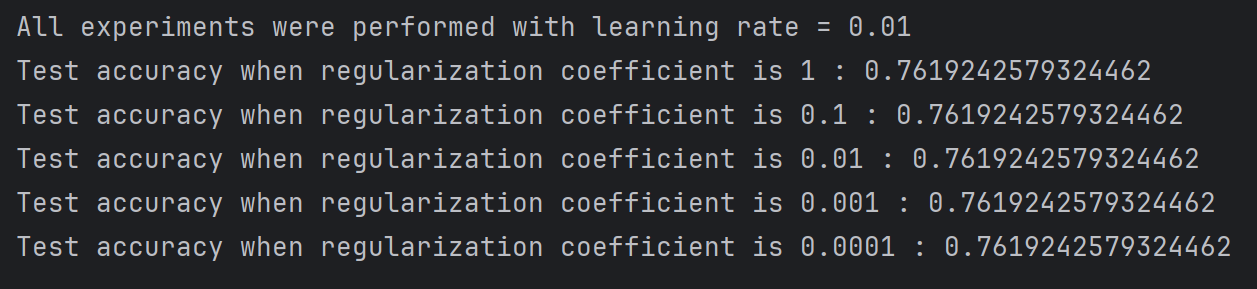
\includegraphics[height=.063\textheight]{./figure/myplotS12.png}
			\caption{Fixing the learning rate}
		\end{subfigure}
		\begin{subfigure}{.45\textwidth}
			\centering
			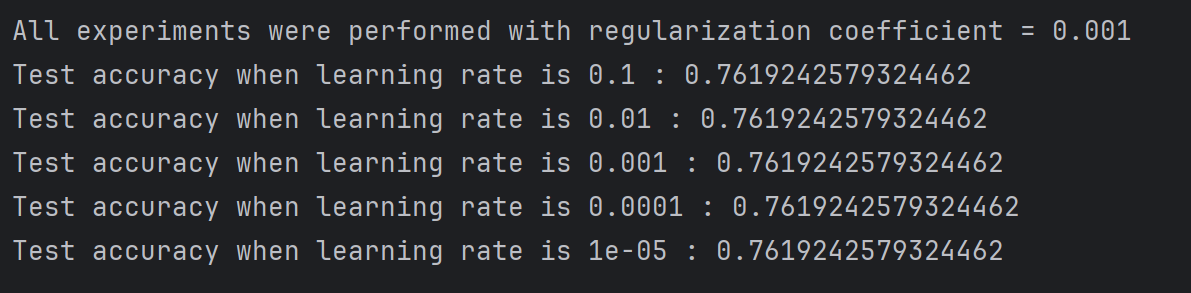
\includegraphics[height=.063\textheight]{./figure/myplotS13.png}
			\caption{Fixing the regularization coefficient}
		\end{subfigure}
		\caption{Result on different learning rate and regularization coefficient}
	\end{figure}
	
	However, the choice of regularization parameter is typically crucial for the model's generalization ability. A larger regularization coefficient helps to constrain the complexity of the model, effectively preventing overfitting, while a smaller regularization coefficient allows the model to capture more details in the data, improving its fitting ability on the training set. In practical tasks, selecting the appropriate regularization coefficient requires careful optimization based on cross-validation and the characteristics of the dataset.
	
	Overall, the experimental results suggest that neither adjustments to the learning rate nor modifications to the regularization coefficient significantly impacted the model's test accuracy. This indicates that the current model's performance may rely more heavily on data characteristics or other hyperparameters (such as the design of the loss function or feature preprocessing). In future experiments, it would be beneficial to expand the range of learning rates and regularization parameters or investigate the influence of other hyperparameters to further improve model performance and gain deeper insights into the model's behavior and characteristics. The code is shown as \verb|SimpleSVM.py|.
	
	\begin{figure}[htbp]
		\centering
		\begin{subfigure}{.45\textwidth}
			\centering
			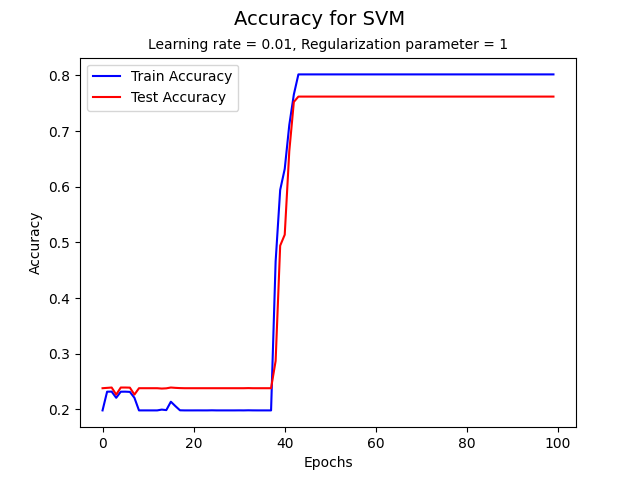
\includegraphics[width=.9\textwidth]{./figure/myplotS2.png}
			\caption{Regularization coefficient = 1}
		\end{subfigure}
		\begin{subfigure}{.45\textwidth}
			\centering
			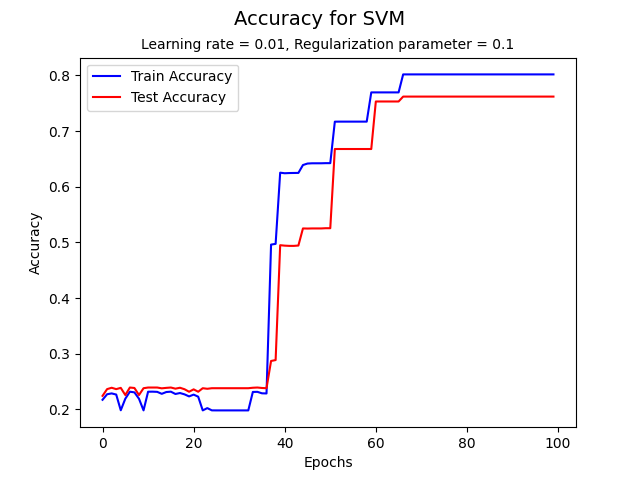
\includegraphics[width=.9\textwidth]{./figure/myplotS3.png}
			\caption{Regularization coefficient = 0.1}
		\end{subfigure}
		\begin{subfigure}{.45\textwidth}
			\centering
			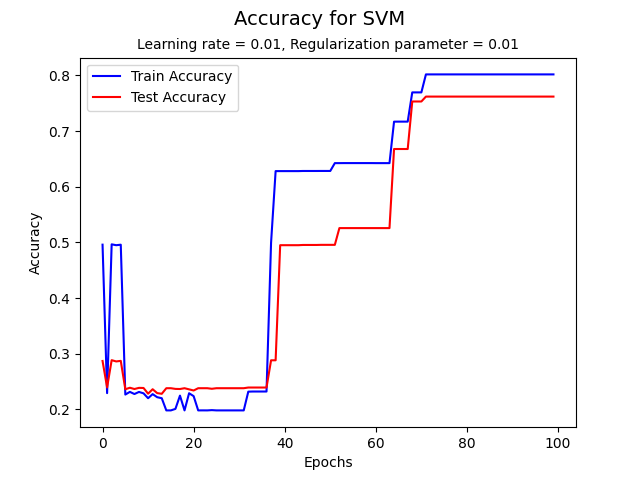
\includegraphics[width=.9\textwidth]{./figure/myplotS4.png}
			\caption{Regularization coefficient = 0.01}
		\end{subfigure}
		\begin{subfigure}{.45\textwidth}
			\centering
			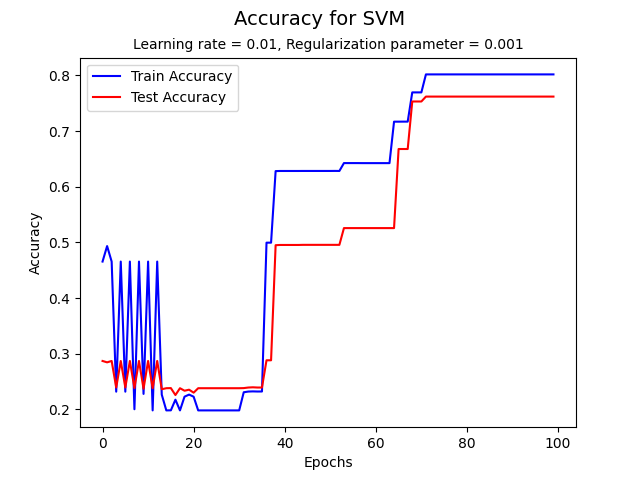
\includegraphics[width=.9\textwidth]{./figure/myplotS5.png}
			\caption{Regularization coefficient = 0.001}
		\end{subfigure}
		\caption{Accuracy curve on different regularization coefficient with learning rate = 0.01}
	\end{figure}
	
	\begin{figure}[htbp]
		\centering
		\begin{subfigure}{.45\textwidth}
			\centering
			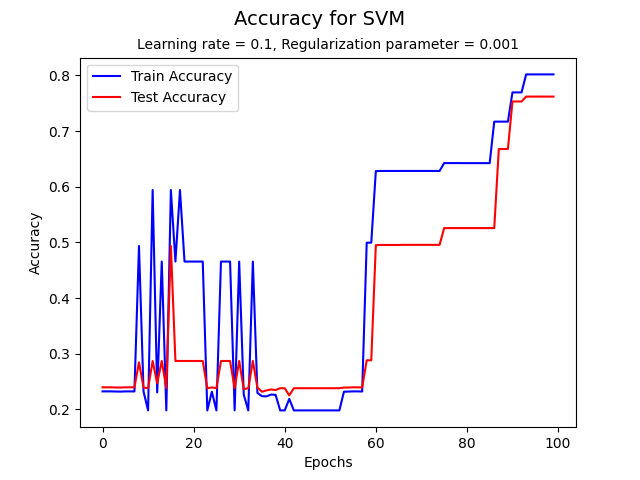
\includegraphics[width=.9\textwidth]{./figure/myplotS7.png}
			\caption{Learning rate = 0.1}
		\end{subfigure}
		\begin{subfigure}{.45\textwidth}
			\centering
			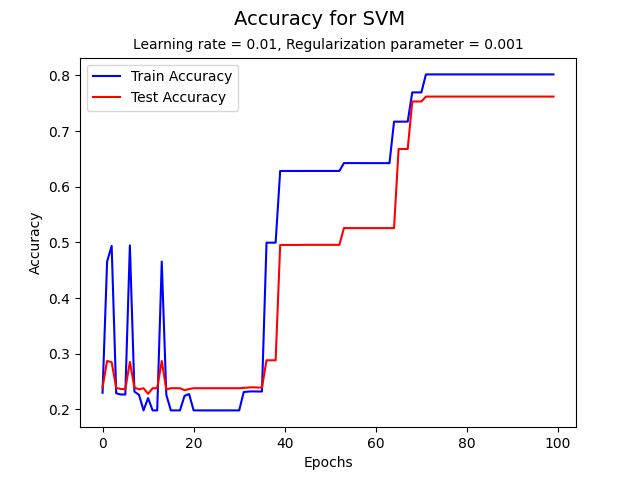
\includegraphics[width=.9\textwidth]{./figure/myplotS8.png}
			\caption{Learning rate = 0.01}
		\end{subfigure}
		\begin{subfigure}{.45\textwidth}
			\centering
			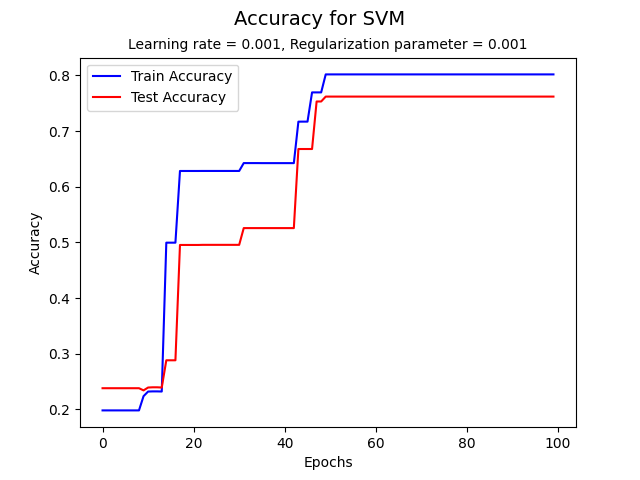
\includegraphics[width=.9\textwidth]{./figure/myplotS9.png}
			\caption{Learning rate = 0.001}
		\end{subfigure}
		\begin{subfigure}{.45\textwidth}
			\centering
			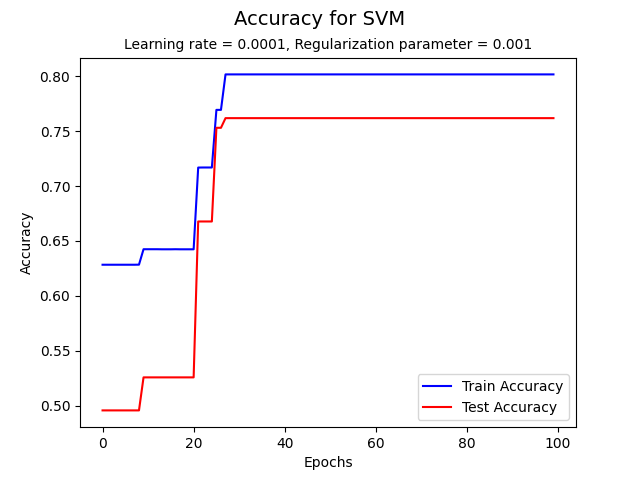
\includegraphics[width=.9\textwidth]{./figure/myplotS10.png}
			\caption{Learning rate = 0.0001}
		\end{subfigure}
		\caption{Accuracy curve on different learning rate with regularization coefficient = 0.001}
	\end{figure}
	
	\subsection{Oversampling and Undersampling}
	
	After implementing optimization strategies such as momentum and learning rate decay, we observed a significant improvement in the test accuracy during the experiments. However, it is regrettable that the prediction results revealed a clear bias towards one particular class. In other words, the model appeared to predict all samples as belonging to a single label rather than accurately distinguishing between different classes. This phenomenon suggests that dataset imbalance could be a critical factor contributing to the suboptimal performance of the model. To further investigate the impact of data imbalance on model performance, this experiment adopted two strategies: oversampling and undersampling.
	
	In the experiment, we oversampled the minority class by increasing the number of its samples and undersampled the majority class by reducing its sample count to rebalance the dataset. The rebalanced dataset was then used to retrain and test the model. Although the balance of the data distribution was improved to some extent, the test accuracy unexpectedly showed a noticeable decline. With a fixed momentum value of 0.99 and a learning rate decay rate of 0.9, and across various settings of regularization parameters and learning rates, the accuracy remained at a relatively low level, between approximately 34\% and 36\%. This indicates that simply applying oversampling or undersampling does not effectively improve model performance. On the contrary, these strategies might disrupt the original characteristics of the data, leading to a decline in classification ability.
	
	\begin{figure}[htbp]
		\centering
		\begin{subfigure}{.5\textwidth}
			\centering
			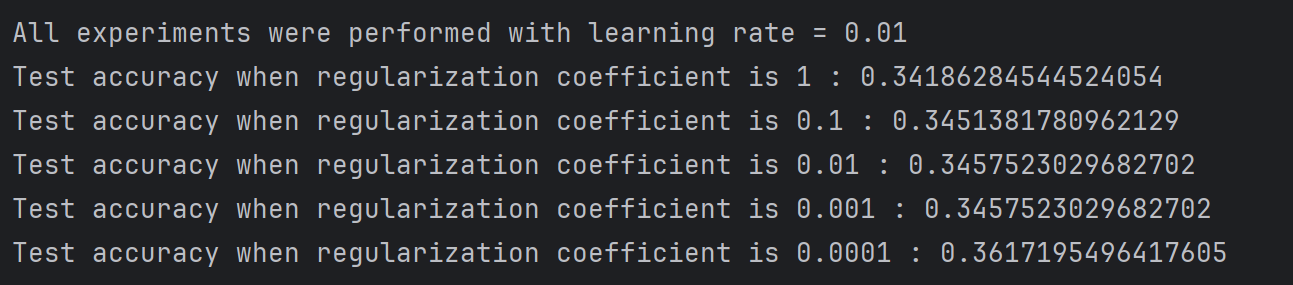
\includegraphics[height=.063\textheight]{./figure/myplotFS12.png}
			\caption{Fixing the learning rate}
		\end{subfigure}
		\begin{subfigure}{.45\textwidth}
			\centering
			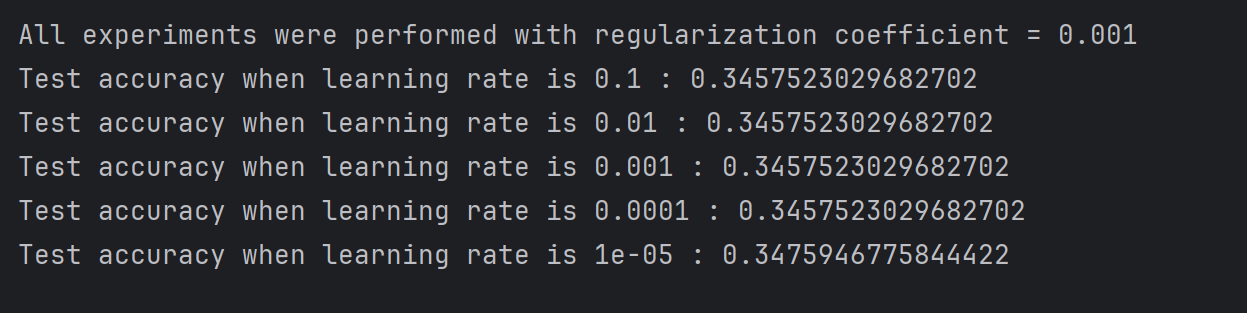
\includegraphics[height=.063\textheight]{./figure/myplotFS13.png}
			\caption{Fixing the regularization coefficient}
		\end{subfigure}
		\caption{Result on different learning rate and regularization coefficient}
	\end{figure}
	
	This phenomenon could be attributed to several factors. First, oversampling may introduce excessive redundant information, causing the model to overfit the minority class. Second, undersampling reduces the number of majority class samples, which might result in insufficient learning of majority class features by the model. Additionally, the fundamental nature of the data imbalance problem might not be solvable solely by adjusting sample quantities. More sophisticated strategies, such as data augmentation using generative adversarial networks (GANs) or designing weighted loss functions, might be required for more effective optimization.
	
	Overall, the experimental results indicate that oversampling and undersampling had limited effectiveness in this study. These approaches not only failed to address the prediction bias problem but also negatively impacted the overall accuracy. This finding underscores the importance of designing more robust and adaptable solutions to tackle data imbalance issues, providing valuable insights and direction for future research. The code is shown as \verb|FilterSVM.py|.
	
	\begin{figure}[htbp]
		\centering
		\begin{subfigure}{.45\textwidth}
			\centering
			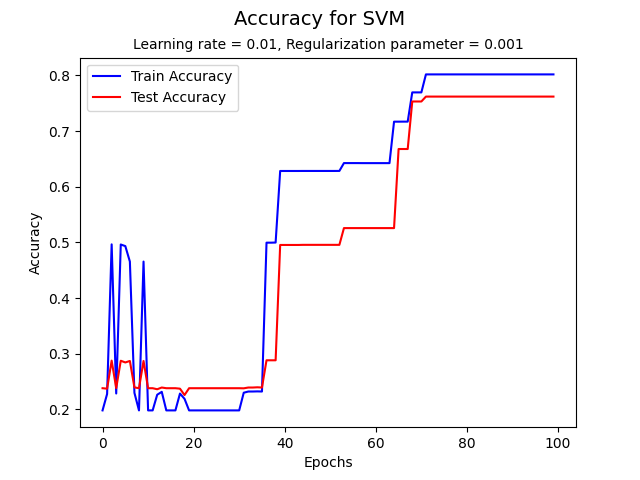
\includegraphics[width=.9\textwidth]{./figure/myplotS1.png}
			\caption{Before oversampling and undersampling}
		\end{subfigure}
		\begin{subfigure}{.45\textwidth}
			\centering
			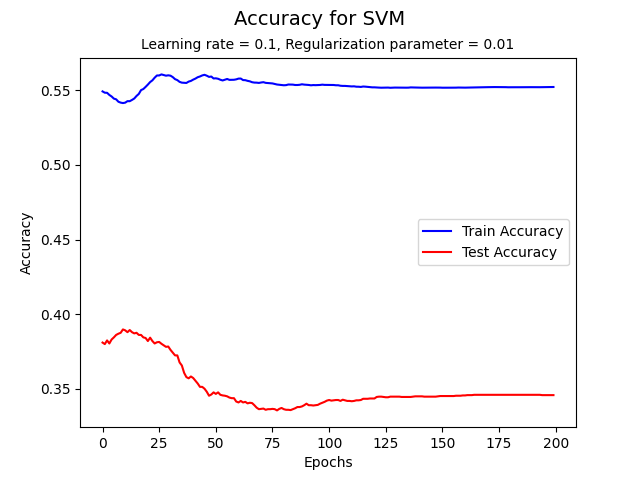
\includegraphics[width=.9\textwidth]{./figure/myplotFS1.png}
			\caption{After oversampling and undersampling}
		\end{subfigure}
		\caption{Comparison of results before and after using oversampling and undersampling}
	\end{figure}
	
	\subsection{Feature Selection}
	
	During the experiment, we conducted an in-depth study of various feature combinations to evaluate the impact of feature selection on the predictive performance of the Support Vector Machine (SVM) model. The primary goal was to identify and select key features that could improve the model's classification accuracy on the test dataset. However, as revealed in the previous section, relying solely on simple feature engineering techniques may not yield remarkable results.
	
	\begin{figure}[htbp]
		\centering
		\begin{subfigure}{.48\textwidth}
			\centering
			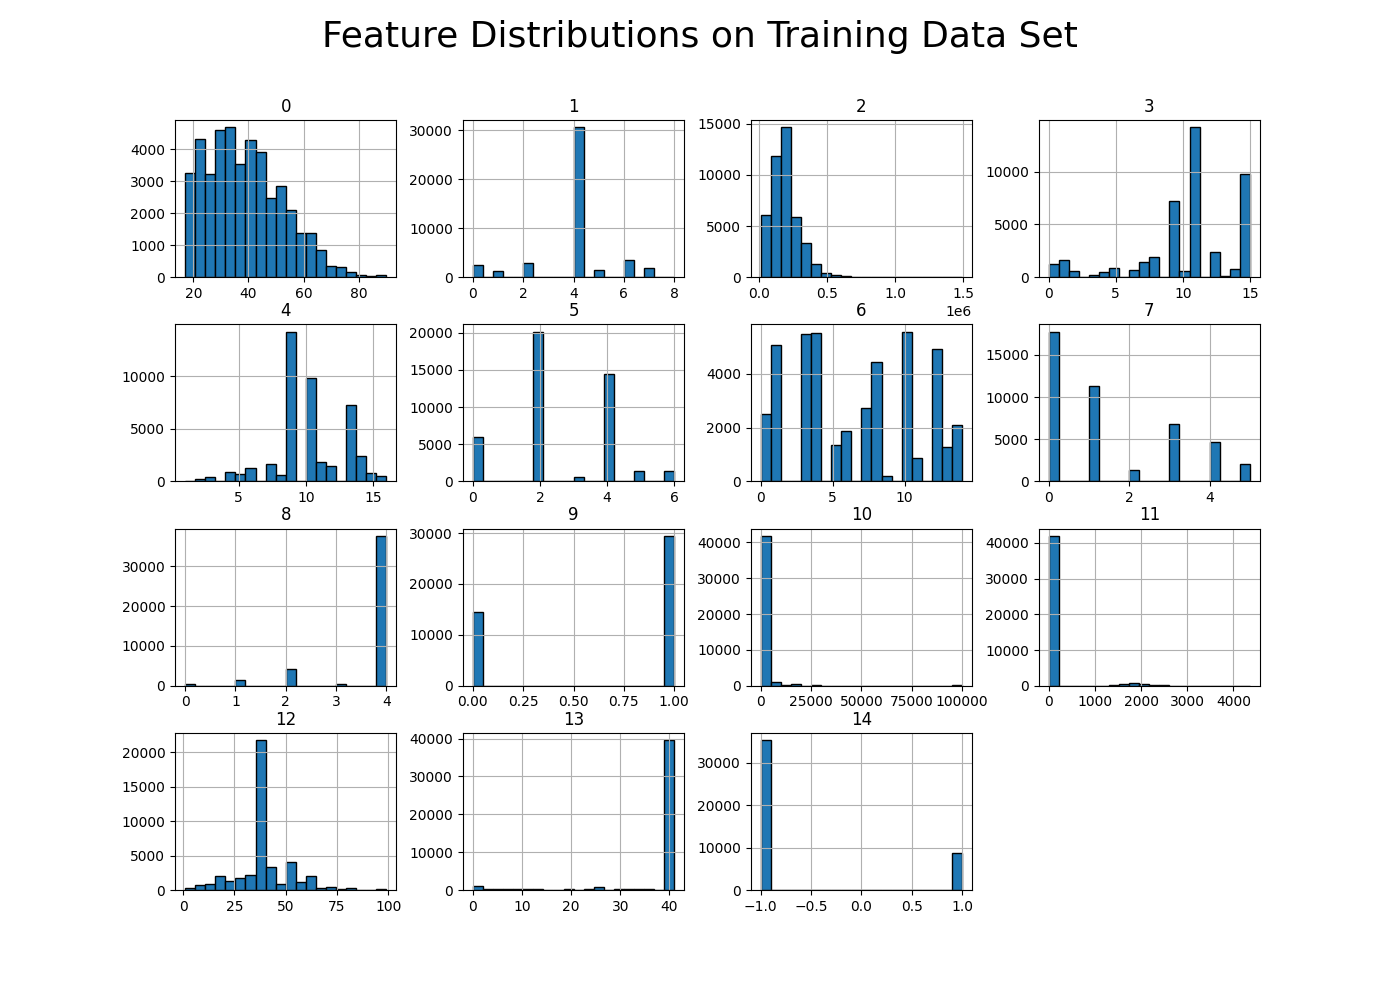
\includegraphics[width=\textwidth]{./figure/myplotF1.png}
			\caption{Feature distribution on training set}
		\end{subfigure}
		\begin{subfigure}{.48\textwidth}
			\centering
			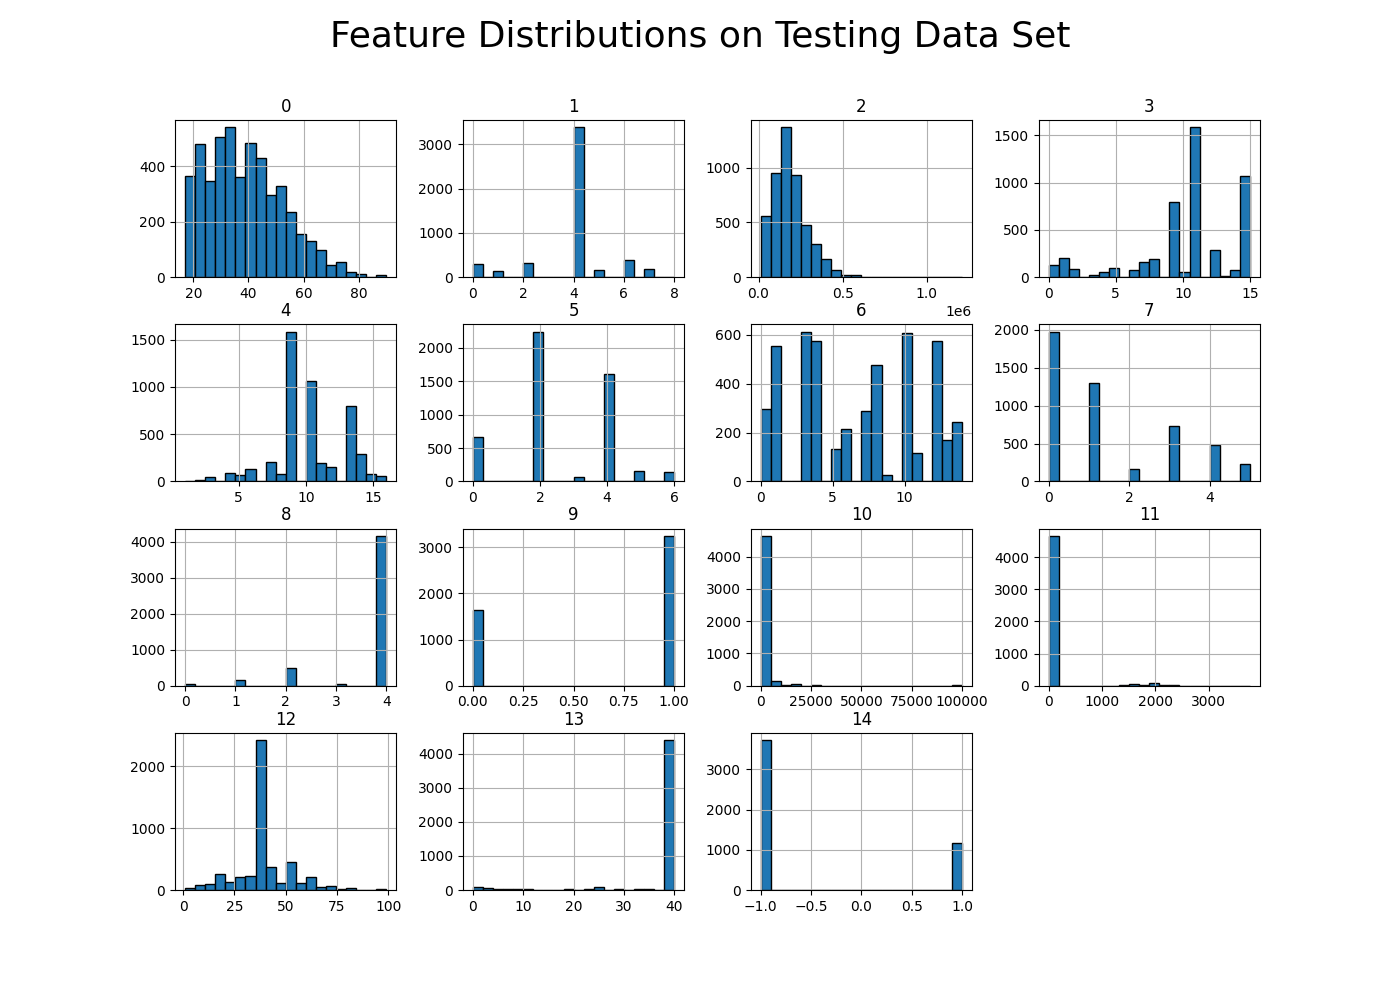
\includegraphics[width=\textwidth]{./figure/myplotF2.png}
			\caption{Feature distribution on testing set}
		\end{subfigure}
		\caption{Feature distribution on the provided dataset}
	\end{figure}
	
	Based on the distribution of different features and through a series of experiments, we identified that ``\textbf{Relationship}'' and ``\textbf{Capital-loss}'' were critical features for the model's performance. When the model used only these two features, it achieved an accuracy of 49.48\% on the test dataset. We then attempted to include ``\textbf{Native-country}'' as an additional feature. While this increased the dimensionality of the feature set, it did not improve the test accuracy, which remained at 49.48\%. Expanding the feature set further to include ``\textbf{Fnlwgt}'', forming a total of four features, still failed to surpass this accuracy level but managed to maintain it at 49.48\% without degradation. These results identified \textbf{Relationship}, \textbf{Capital-loss}, \textbf{Native-country}, and \textbf{Fnlwgt} as the key features.
	
	In contrast, other feature combinations yielded suboptimal performance. For instance, selecting ``\textbf{Education-num}'', ``\textbf{Marital-status}'', and ``\textbf{Sex}'' as features resulted in a test accuracy of only 34.74\%. When using ``\textbf{Fnlwgt}'', ``\textbf{Education}'', ``\textbf{Occupation}'', and ``\textbf{Hours-per-week}'', the accuracy showed a modest improvement to 36.60\%. These findings highlight that not all features contribute equally to the classification task.
	
	Although the selection of critical features optimized the model to some extent, the overall accuracy remained below 50\%. Nevertheless, compared to a baseline model without feature selection, the accuracy improved by approximately 70\%, indicating that feature selection does have a significant positive impact on model performance. However, it is also evident that the model's performance remains constrained by other factors, such as data imbalance or the model's capacity limitations.
	
	In summary, while feature selection can enhance model performance to a certain degree, its effects are limited and insufficient to overcome the performance bottlenecks observed in this experiment. This underscores the importance of combining data preprocessing, feature engineering, and optimization techniques for achieving better results, providing valuable insights and direction for future research. The code is shown as \verb|FeatureSVM.py|.
	
	\begin{figure}[htbp]
		\centering
		\begin{subfigure}{.32\textwidth}
			\centering
			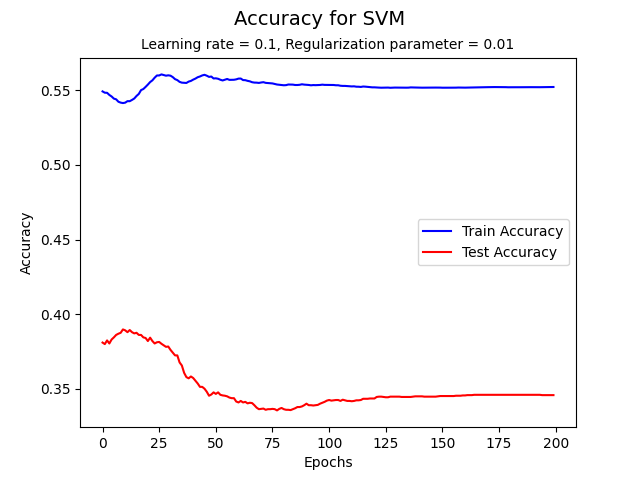
\includegraphics[width=.9\textwidth]{./figure/myplotFS1.png}
			\caption{Without selecting features}
		\end{subfigure}
		\begin{subfigure}{.32\textwidth}
			\centering
			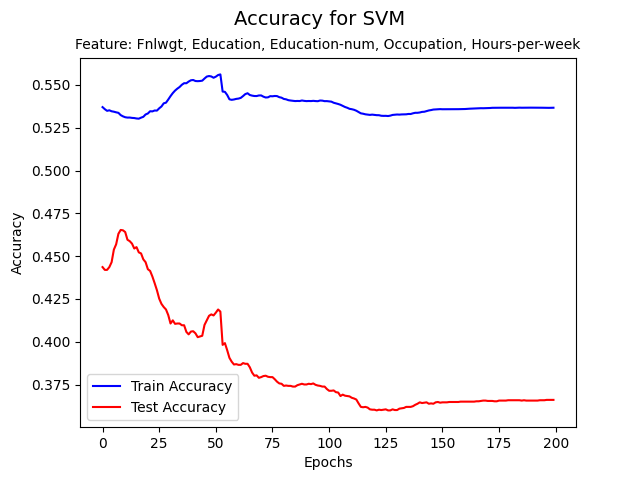
\includegraphics[width=.9\textwidth]{./figure/myplotF7.png}
			\caption{Selecting unrelated features}
		\end{subfigure}
		\begin{subfigure}{.32\textwidth}
			\centering
			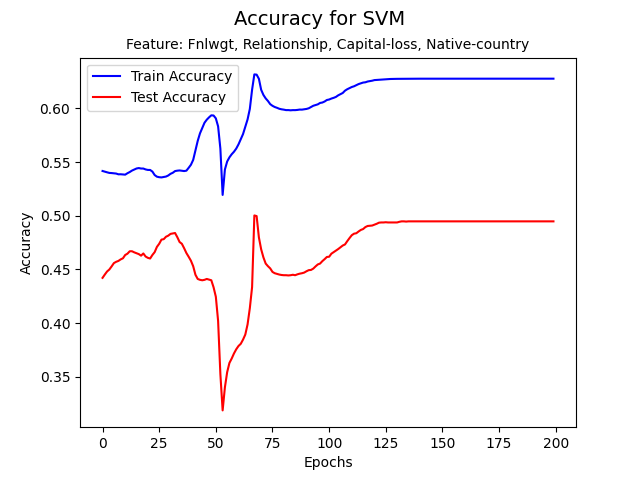
\includegraphics[width=.9\textwidth]{./figure/myplotF5.png}
			\caption{Selecting four key features}
		\end{subfigure}
		\caption{Comparison of results before and after feature selection}
	\end{figure}
	
	\subsection{Comparative Experiment}
	
	To comprehensively analyze the performance of the Support Vector Machine (SVM) implemented in this experiment, we trained both logistic regression (as implemented in Homework 3) and SVM using the same dataset, learning rate, and regularization coefficient. The objective was to explore their classification performance differences under various feature combinations. We designed three experiments as follows: (1) without feature selection; (2) using only the features ``\textbf{Relationship}'' and ``\textbf{Capital-loss}''; (3) using four features: ``\textbf{Relationship}'', ``\textbf{Capital-loss}'', ``\textbf{Native-country}'', and ``\textbf{Fnlwgt}''.
	
	Without feature selection, the test accuracy of logistic regression was 59.12\%, while the accuracy of SVM was 34.58\%. Logistic regression significantly outperformed SVM, likely due to its stronger ability to capture linear relationships in the full feature space. In contrast, SVM encountered limitations when dealing with high-dimensional features, such as the imbalance in data distribution or the influence of redundant features on the hyperplane.
	
	When only the two key features, ``\textbf{Relationship}'' and ``\textbf{Capital-loss}'' were used, the test accuracy of logistic regression decreased to 50.62\%, while SVM achieved an accuracy of 49.48\%. At this point, the performance gap between the two methods narrowed. Compared to the experiment in the full feature space, logistic regression exhibited a notable decline in accuracy, whereas SVM showed an improvement. This indicates that SVM is less reliant on noise and can benefit from the reduction in feature dimensions.
	
	Expanding to four features, logistic regression's test accuracy further dropped to 47.41\%, while SVM's accuracy remained stable at 49.48\%. The decline in logistic regression performance suggests that the newly added features contributed little to the model or even introduced redundancy. Logistic regression appeared to be more sensitive to this redundancy, leading to a decrease in performance. On the other hand, SVM, by focusing on support vectors, effectively mitigated the impact of redundant features.
	
	The experimental results reveal that logistic regression performed better than SVM in the full feature space, likely due to its strong adaptability to the linear relationships in the data. However, after feature selection, SVM demonstrated more stable performance, particularly when key features were extracted, showcasing its robustness. This comparison highlights that feature selection plays a more significant role in optimizing the performance of SVM, while logistic regression shows greater advantages in high-dimensional data. The differences in model performance also reflect the interplay between data distribution characteristics and model capabilities, providing valuable insights for further model optimization. The code is shown as \verb|Logistic.py|.
	
	\begin{figure}[htbp]
		\centering
		\begin{subfigure}{.32\textwidth}
			\centering
			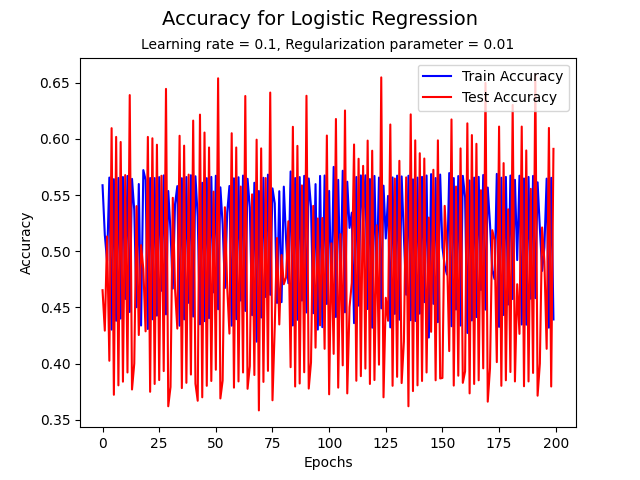
\includegraphics[width=.9\textwidth]{./figure/myplotL1.png}
			\caption{Without selecting features}
		\end{subfigure}
		\begin{subfigure}{.32\textwidth}
			\centering
			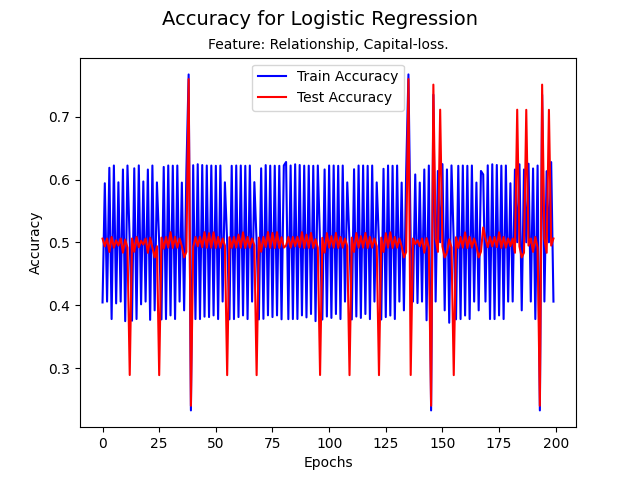
\includegraphics[width=.9\textwidth]{./figure/myplotL2.png}
			\caption{Selecting two key features}
		\end{subfigure}
		\begin{subfigure}{.32\textwidth}
			\centering
			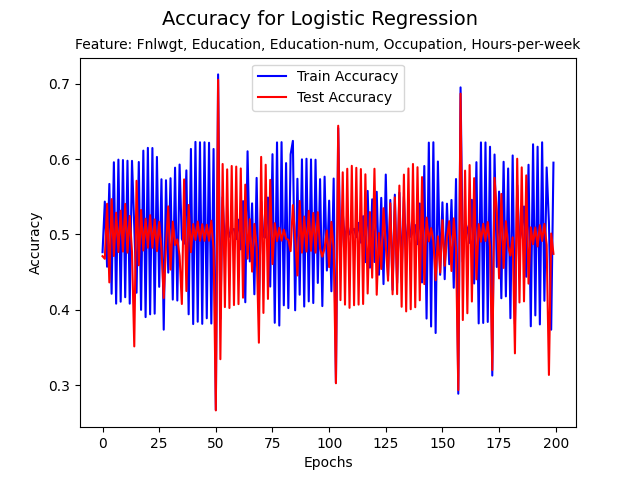
\includegraphics[width=.9\textwidth]{./figure/myplotL3.png}
			\caption{Selecting four key features}
		\end{subfigure}
		\caption{Accuracy curve on logistic regression with learning rate = 0.01 and regularization coefficient = 0.001}
	\end{figure}
	
	\section{Conclusion}
	
	This experiment conducted an in-depth analysis of the classification performance of Support Vector Machines (SVM) on datasets containing both numerical and categorical features. The results indicate that learning rate and regularization coefficient have a limited impact on model performance, although they could have a significant influence in more complex datasets or different model structures. Additionally, the experiment found that simple oversampling and undersampling strategies failed to effectively improve model performance, highlighting the need for more refined approaches to handle imbalanced datasets.
	
	Feature selection experiments revealed that different feature combinations significantly affect model performance, but the overall accuracy did not exceed 50\%. This suggests that while feature selection helps improve performance to some extent, its impact is limited. Comparative experiments demonstrated performance differences between logistic regression and SVM under various feature combinations. The findings show that feature selection plays a critical role in optimizing SVM performance, whereas logistic regression exhibits greater advantages in high-dimensional data.
	
	In summary, the experiment validates the effectiveness of SVM in classification tasks and underscores several factors to consider in practical applications. These insights provide valuable references for further research and model optimization.
	
	\let\cleardoublepage\clearpage
	
	\begin{thebibliography}{99}  
		\bibitem{ref1} 谢文睿, 秦州, 贾彬彬. 机器学习公式详解[M]. 第2版. 北京:人民邮电出版社, 2023 :77-99.
		\bibitem{ref2} 张伟楠, 赵寒烨, 俞勇. 动手学机器学习[M]. 第1版. 北京:人民邮电出版社, 2023 :150-166.
		\bibitem{ref3} 周志华. 机器学习[M]. 第1版. 北京:清华大学出版社, 2016 :121-144.
		\bibitem{ref4} Amari S. Backpropagation and stochastic gradient descent method[J]. Neurocomputing, 1993, 5(4-5): 185-196.
		\bibitem{ref5} Ardeshir N, Sanford C, Hsu D J. Support vector machines and linear regression coincide with very high-dimensional features[J]. Advances in Neural Information Processing Systems, 2021, 34: 4907-4918.
		\bibitem{ref6} Aston Zhang, Zachary C. Lipton, Mu Li, Alexander J. Smola. 动手学机器学习 PyTorch版[M]. Xiaoting He, Rachel Hu. 第1版. 北京:人民邮电出版社, 2023 :311-368.
		\bibitem{ref7} Bach M, Werner A, Żywiec J, et al. The study of under-and over-sampling methods' utility in analysis of highly imbalanced data on osteoporosis[J]. Information Sciences, 2017, 384: 174-190.
		\bibitem{ref8} Bottou L. Large-scale machine learning with stochastic gradient descent[C]//Proceedings of COMPSTAT'2010: 19th International Conference on Computational StatisticsParis France, August 22-27, 2010 Keynote, Invited and Contributed Papers. Physica-Verlag HD, 2010: 177-186.
		\bibitem{ref9} Chauhan V K, Dahiya K, Sharma A. Problem formulations and solvers in linear SVM: a review[J]. Artificial Intelligence Review, 2019, 52: 803-855.
		\bibitem{ref10} Cutkosky A, Mehta H. Momentum improves normalized sgd[C]//International conference on machine learning. PMLR, 2020: 2260-2268.
		\bibitem{ref11} Ge R, Kakade S M, Kidambi R, et al. The step decay schedule: A near optimal, geometrically decaying learning rate procedure for least squares[J]. Advances in neural information processing systems, 2019, 32.
		\bibitem{ref12} Liu S, Zhang J, Xiang Y, et al. A study of data pre-processing techniques for imbalanced biomedical data classification[J]. International Journal of Bioinformatics Research and Applications, 2020, 16(3): 290-318.
		\bibitem{ref13} Loshchilov I. Decoupled weight decay regularization[J]. arXiv preprint arXiv:1711.05101, 2017.
		\bibitem{ref14} Xiaolong X U, Wen C, Yanfei S U N. Over-sampling algorithm for imbalanced data classification[J]. Journal of Systems Engineering and Electronics, 2019, 30(6): 1182-1191.
	\end{thebibliography}
	
\end{document}